%
%  MP_talk.tex
%
%  Created by Steven Harms (HOME) on 2011-07-26.
%  Copyright (c) 2011 Steven G. Harms. All rights reserved.
%
\documentclass[slidestop,compress,mathserif]{beamer}
% \documentclass[slidestop,compress,mathserif, slidesonly]{beamer}
% Toggle between 'notes' and no notes to display or undisplay notes pages

% \usepackage[bars]{beamerthemetree}
\usetheme{PaloAlto}
\usecolortheme{seahorse}

% Use utf-8 encoding for foreign characters
\usepackage[utf8]{inputenc}

% Surround parts of graphics with box
\usepackage{boxedminipage}

% Package for including code in the document
\usepackage{listings}

% This is now the recommended way for checking for PDFLaTeX:
\usepackage{ifpdf}

% Support for handouts
\usepackage{pgfpages}
% \pgfpagesuselayout{4 on 1}[a4paper,border shrink=5mm]

\ifx\pdftexversion\undefined
\usepackage[dvips]{graphicx}
\else
\usepackage{graphicx}
\DeclareGraphicsRule{*}{mps}{*}{}
\fi
\title{Practical Metaprogramming:  Modeling Thought}
\author{ Steven G. Harms }

\date{2011-08-12}

\begin{document}

\ifpdf
\DeclareGraphicsExtensions{.pdf, .jpg, .tif}
\else
\DeclareGraphicsExtensions{.eps, .jpg}
\fi


\section{Introduction} % (fold)
\label{sec:introduction}
\begin{frame}
	\maketitle
\end{frame}

\subsection{Administration}
\begin{frame}
	\frametitle{Contact Me!}
	\begin{center}
		Steven G. Harms \\
		\vskip 1.25cm
		Physically:  San Francisco, CA\\
		Email:  \texttt{lsrcv@sgharms.oib.com} \\
		Twitter / GitHub:  \texttt{sgharms} \\
		G+
	\end{center}
\end{frame}
\note{
Good afternoon, I want to welcome you all to the first day of Lone Star Ruby
Conference V. 
}

\begin{frame}
	\frametitle{Austin}
	\begin{center}
		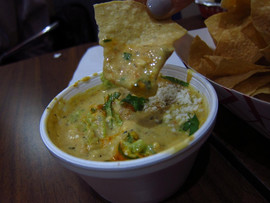
\includegraphics[scale=0.75]{img/queso.JPG}	
		\vskip 0.5cm
		\emph{Austin has many charms.  This is from Torchy's}
	\end{center}
\end{frame}
\note{
It's great to be back here in Austin. I've lived here for over
eight years off and on and love this town, its vibrant Ruby community, and
creativity with turning cheese into a soup that you put chips in. If you don't
know what I'm talking about, talk to me later and we'll get you set up
properly.
}


\subsection{Overview}

\begin{frame}
	\frametitle{What We'll Cover}
	\begin{center}
		Practical Metaprogramming:  ``Modeling Thought''
	\end{center}
\end{frame}
\note
{
\tiny
\begin{itemize}
	\item \emph{Practical Metaprogramming}
	\item Magic of MP
	\begin{itemize}
		\tiny
		\item Short intro cycle
		\item Possibly why we start Ruby in the first place
	\end{itemize}
	\item Poll
	\begin{itemize}
		\tiny
		\item Who was introduced to Ruby as a side effect of ``Hey isn't it neat that Ruby can do this?''
		\item How many of you have no idea what I'm talking about when I say ``metaprogramming?''; you will also be able to benefit from this discussion
	\end{itemize}
	\item Introduced as a gimmick
	\item This talk can	help you dispel FUD, feel confident in metaprogramming
	\item I	will not have the ability to cover all the MP code blocks
	\item Modeling thought: a technique or a dispotition which is designed to help intermediate metaprogrammers evaluate whether an MP-based
	solution is the right solution for them.  While not infallible, pretty good.
\end{itemize}
\normalsize
}

\begin{frame}
	\frametitle{Goals}
	\begin{enumerate}
		\item Reflect upon how we learn MP in the Ruby community
		\pause
		\item Demonstrate MP's ubiquity:  you can't \emph{not} learn this
		\pause
		\item Advise when you should reach for the MP ``hammer''
		\pause
		\item Provide a real-world example of thinking in terms of MP
		\pause
		\item Give you the confidence to use MP \textbf{boldly}
	\end{enumerate}
\end{frame}
\note{
That's the lay of the land for this talk. If you're thinking this talk might
not be for you, then you're welcome to hop over to the other track.
}

\begin{frame}
	\frametitle{Intermission}
	\begin{center}
		\texttt{INTERMISSION}
	\end{center}
\end{frame}

\begin{frame}
	\frametitle{Socially Awkward Penguin}
	\begin{center}
		
\includegraphics[scale=0.3]{img/sap.png}
	\end{center}
\end{frame}
\note{
Whew, I'm glad we only lost those few.
}

\begin{frame}
	\frametitle{End Slide if Everyone Leaves}
	\begin{center}
		
\includegraphics[scale=0.15]{img/forever_alone.png}
		\vskip 0.5cm
		\emph{Forever Alone{\ldots}}
	\end{center}
\end{frame}


\section{Practical MP} % (fold)
\label{sub:practical_metaprogramming}

\subsection{Early Exposure} % (fold)
\label{sub:early_exposure}

\begin{frame}
	\frametitle{``Practical Metaprogramming:  First Contact''}
	
\includegraphics[scale=0.55]{img/first_contact.jpg} \\
	\emph{\ldots and is it to be called an ``eigenclass'' or a ``singleton class,'' ma'am?}
\end{frame}
\note{
	\begin{itemize}
		\item How we, as a community, educate our newest members in the technology of metaprogramming.
		\item ``How do we start exploring MP in Ruby?''
	\end{itemize}
}

\begin{frame} \frametitle{To Metaprogramming via Ruby}
	\texttt{attr\_*} \emph{Page 30}
	\vskip 0.5cm
	\begin{center}
		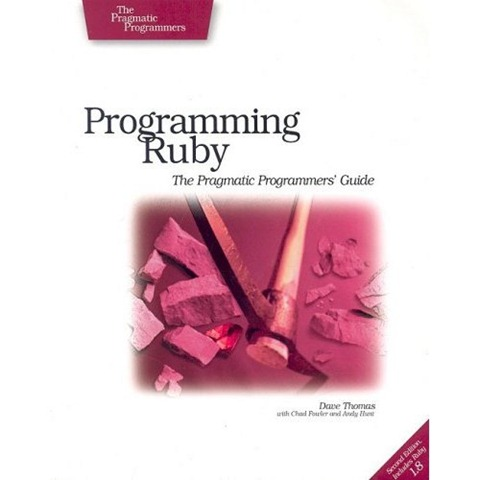
\includegraphics[scale=0.45]{img/ruby_pickaxe.jpg}
	\end{center}
\end{frame}
\note{
	\begin{itemize}
		\item Page thrity of the PickAxe book
		\item \texttt{attr\_reader, attr\_writer, and attr\_accessor}
	\end{itemize}
}

\begin{frame}
	\frametitle{Dynamic Getter / Setter Generation}
	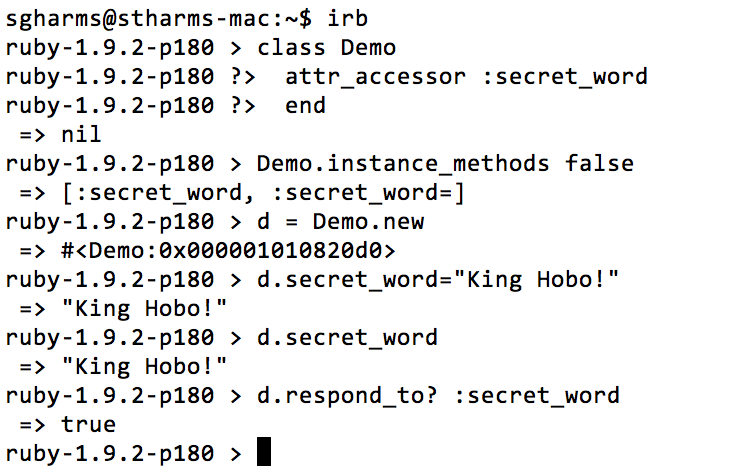
\includegraphics[scale=0.45]{img/attr_demo_1.png}
\end{frame}

\begin{frame} \frametitle{To Metaprogramming via Rails}
	Rails (\texttt{order.discount=0.5}):  \emph{Page 28}
	\begin{center}
		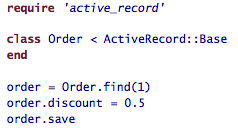
\includegraphics[scale=0.55]{img/awdwr_mp.png}
	\end{center}
\end{frame}
\note{
	\begin{itemize}
		\item Ruby \emph{via Rails}
		\item Page 28 AWDWR
		\item ORM calculation
	\end{itemize}
}

\begin{frame}
	\frametitle{Practical Metaprogramming}
	\begin{itemize}
		\item \texttt{attr\_*}:  \emph{Page 30}
		\item Rails (ORM):  \emph{Page 28}
	\end{itemize}
	\pause
	\vskip 0.5cm
	\emph{But then what?}
\end{frame}
\note{
	\begin{itemize}
		\item Skim the surface
		\item Seems like you have a lot of power
		\item Experimentation
		\item ``First Tier of Metaprogramming Spells''
		\item We tend to use them \emph{impractically} though
	\end{itemize}
}

% subsection early_exposure (end)
\subsection{Intermediate Use} % (fold)
\label{sub:intermediate_use}

\begin{frame}
	\frametitle{Momentary Aside: Terminology}
	``Spells'' and their names derive from \underline{Metaprogramming Ruby} by Paolo ``Nusco'' Perrotta:
	\vskip 0.5cm
	\begin{center}
		\underline{http://ducktypo.blogspot.com/2010/08/} \\
		\underline{metaprogramming-spell-book.html}
	\end{center}
\end{frame}
\note{
	\begin{itemize}
		\item Using the terminology provided by Perrotta
		\item The names are good
		\item As a community needs a common lexicon for reference
		\item There are about 30 of these ``spells,'' as Paolo calls them.
	\end{itemize}
}

\begin{frame}
	\frametitle{``Slightly Impractical Metaprogramming:''  Open Classes}
	\begin{itemize}
		\item Open Classes
	\end{itemize}
		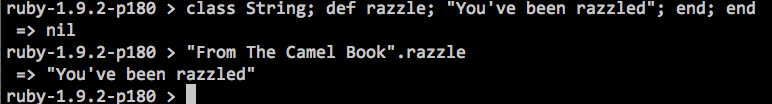
\includegraphics[scale=0.42]{img/open_class.png}
\end{frame}
\note{
	\begin{itemize}
		\item Starts here
		\item You can add methods to an existing \textbf{core} class
		\item ``Open Class'' spell
	\end{itemize}
}


\begin{frame}
	\frametitle{``Slightly Impractical Metaprogramming:''  Kernel Method}
	\begin{itemize}
		\item Open Classes
		\item Kernel Method
	\end{itemize}
		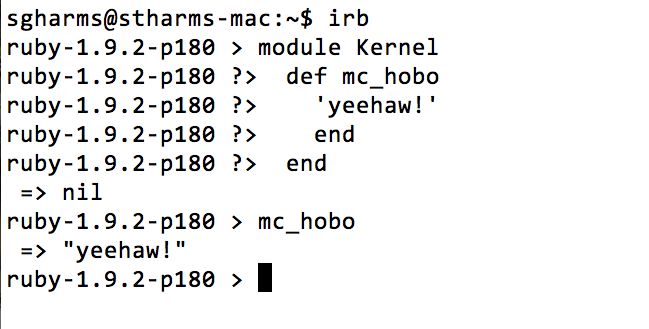
\includegraphics[scale=0.55]{img/kernel_method.png}
\end{frame}
\note{
At this point we're starting to feel some power here. We now see that we can
create methods that behave as if they were core builtins to the language.
}

\begin{frame}
	\frametitle{``Slightly Impractical Metaprogramming:''  Singleton Method}
	\begin{itemize}
		\item Open Classes
		\item Kernel Method
		\item Singleton Method
	\end{itemize}
		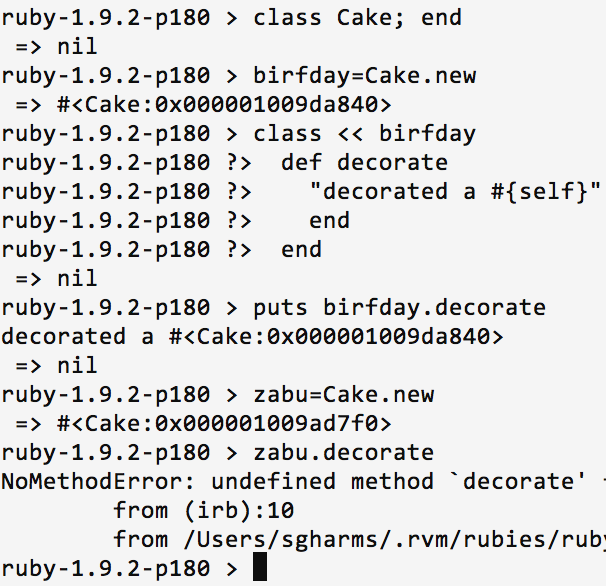
\includegraphics[scale=0.35]{img/singleton_method.png}
\end{frame}
\note{
	\begin{itemize}
		\item Jerks tears from Java programmers
		\item This is undoubtedly the one that makes the pro-Java camp weep.
		\item In compiled languages the definition of a class represents a static contract between the developer and the compiler.
		\item A class is an expression of that contract.
		\item In Ruby, a class is really a namespace expression.
		\item Simple truth that is easy to hear, but hard to \emph{understand}.
		\item \textbf{THIS IS AWESOME}
	\end{itemize}
}

\subsection{Danger Zone} % (fold)
\label{sub:danger_zone}

\begin{frame}
		\frametitle{AWESOMENESS}
		\begin{center}
			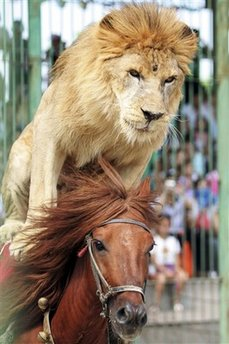
\includegraphics[scale=0.45]{img/lion_horse.jpg} \\
			\emph{-- Credit Unknown}
		\end{center}
\end{frame}
\note{It might not be the most awesome thing ever, which is, of course, a lion riding a horse, but it's still pretty good.}

\begin{frame}
	\frametitle{{\ldots}Or Madness?}
	Incautiously used, these lead to the dangers of MP:
	\begin{itemize}
		\item Opaqueness
		\item Unpredictability
		\item Unsupportability
	\end{itemize}
\end{frame}
\note{This quickly becomes side-effect soup.  So much so that you get elements of doubt.}

\begin{frame}
	\frametitle{Thesis:  F.U.D.}
		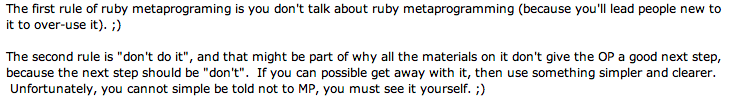
\includegraphics[width=0.98\textwidth, height=0.25\textheight]{img/tim_hates_mp.png}
		\vskip 0.5cm
		\emph{--Tim Connor:  SF Ruby Mailing List}
\end{frame}
\note{
	I had a mail from Tim and his personal views aren't as strong as this, but
he's definitely urging caution over MP's over-use.
}

\begin{frame}
	\frametitle{Antithesis:  anti-F.U.D.}
	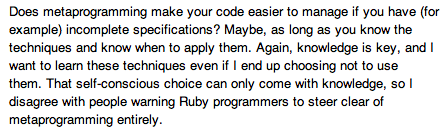
\includegraphics[width=0.98\textwidth, height=0.45\textheight]{img/paolo_anti_fud.png}
	\vskip 0.5cm
	\emph{--Paolo Perrotta, author of Metaprogramming Ruby, in e-mail to Steven Harms}
\end{frame}
\note{
\begin{itemize}
	\item Leaves quite a bit to chance
	\item This attitude implies that we think the material is optional or unimportant.
	\item It is not
\end{itemize}
}

\subsection{Benefits} % (fold)
\label{sub:benefits}

\begin{frame}
	\frametitle{Synthesis:  You Need To Learn This:  Precedent}
	\begin{enumerate}
		\item Virtually all core libraries make use of MP
		\pause
		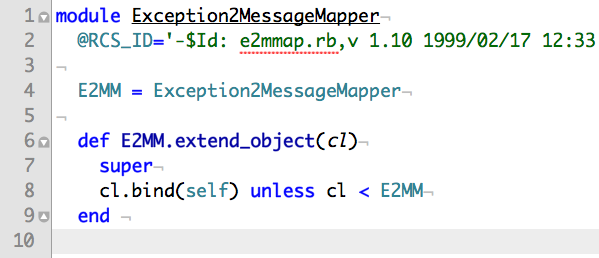
\includegraphics[scale=0.45, width=0.89\textwidth]{img/e2mmap.png}
		\pause
		\item Rails uses MP all over the place
	\end{enumerate}
\end{frame}
\note{
	\begin{itemize}
		\item Part of a community
		\item Precedent
	\end{itemize}
}

\begin{frame}
	\frametitle{Synthesis:  You Need To Learn This:  Your Future}
	\begin{enumerate}
		\item Save yourself a lot of typing
		\pause
		\item Reflect the interior world of your problem domain in your application code
		\pause
		\item Pleasant surprises
	\end{enumerate}
\end{frame}
\note{ \textbf{How will I know when to use MP?}}

\begin{frame}
	\frametitle{How Will I Know?}
	\begin{center}
		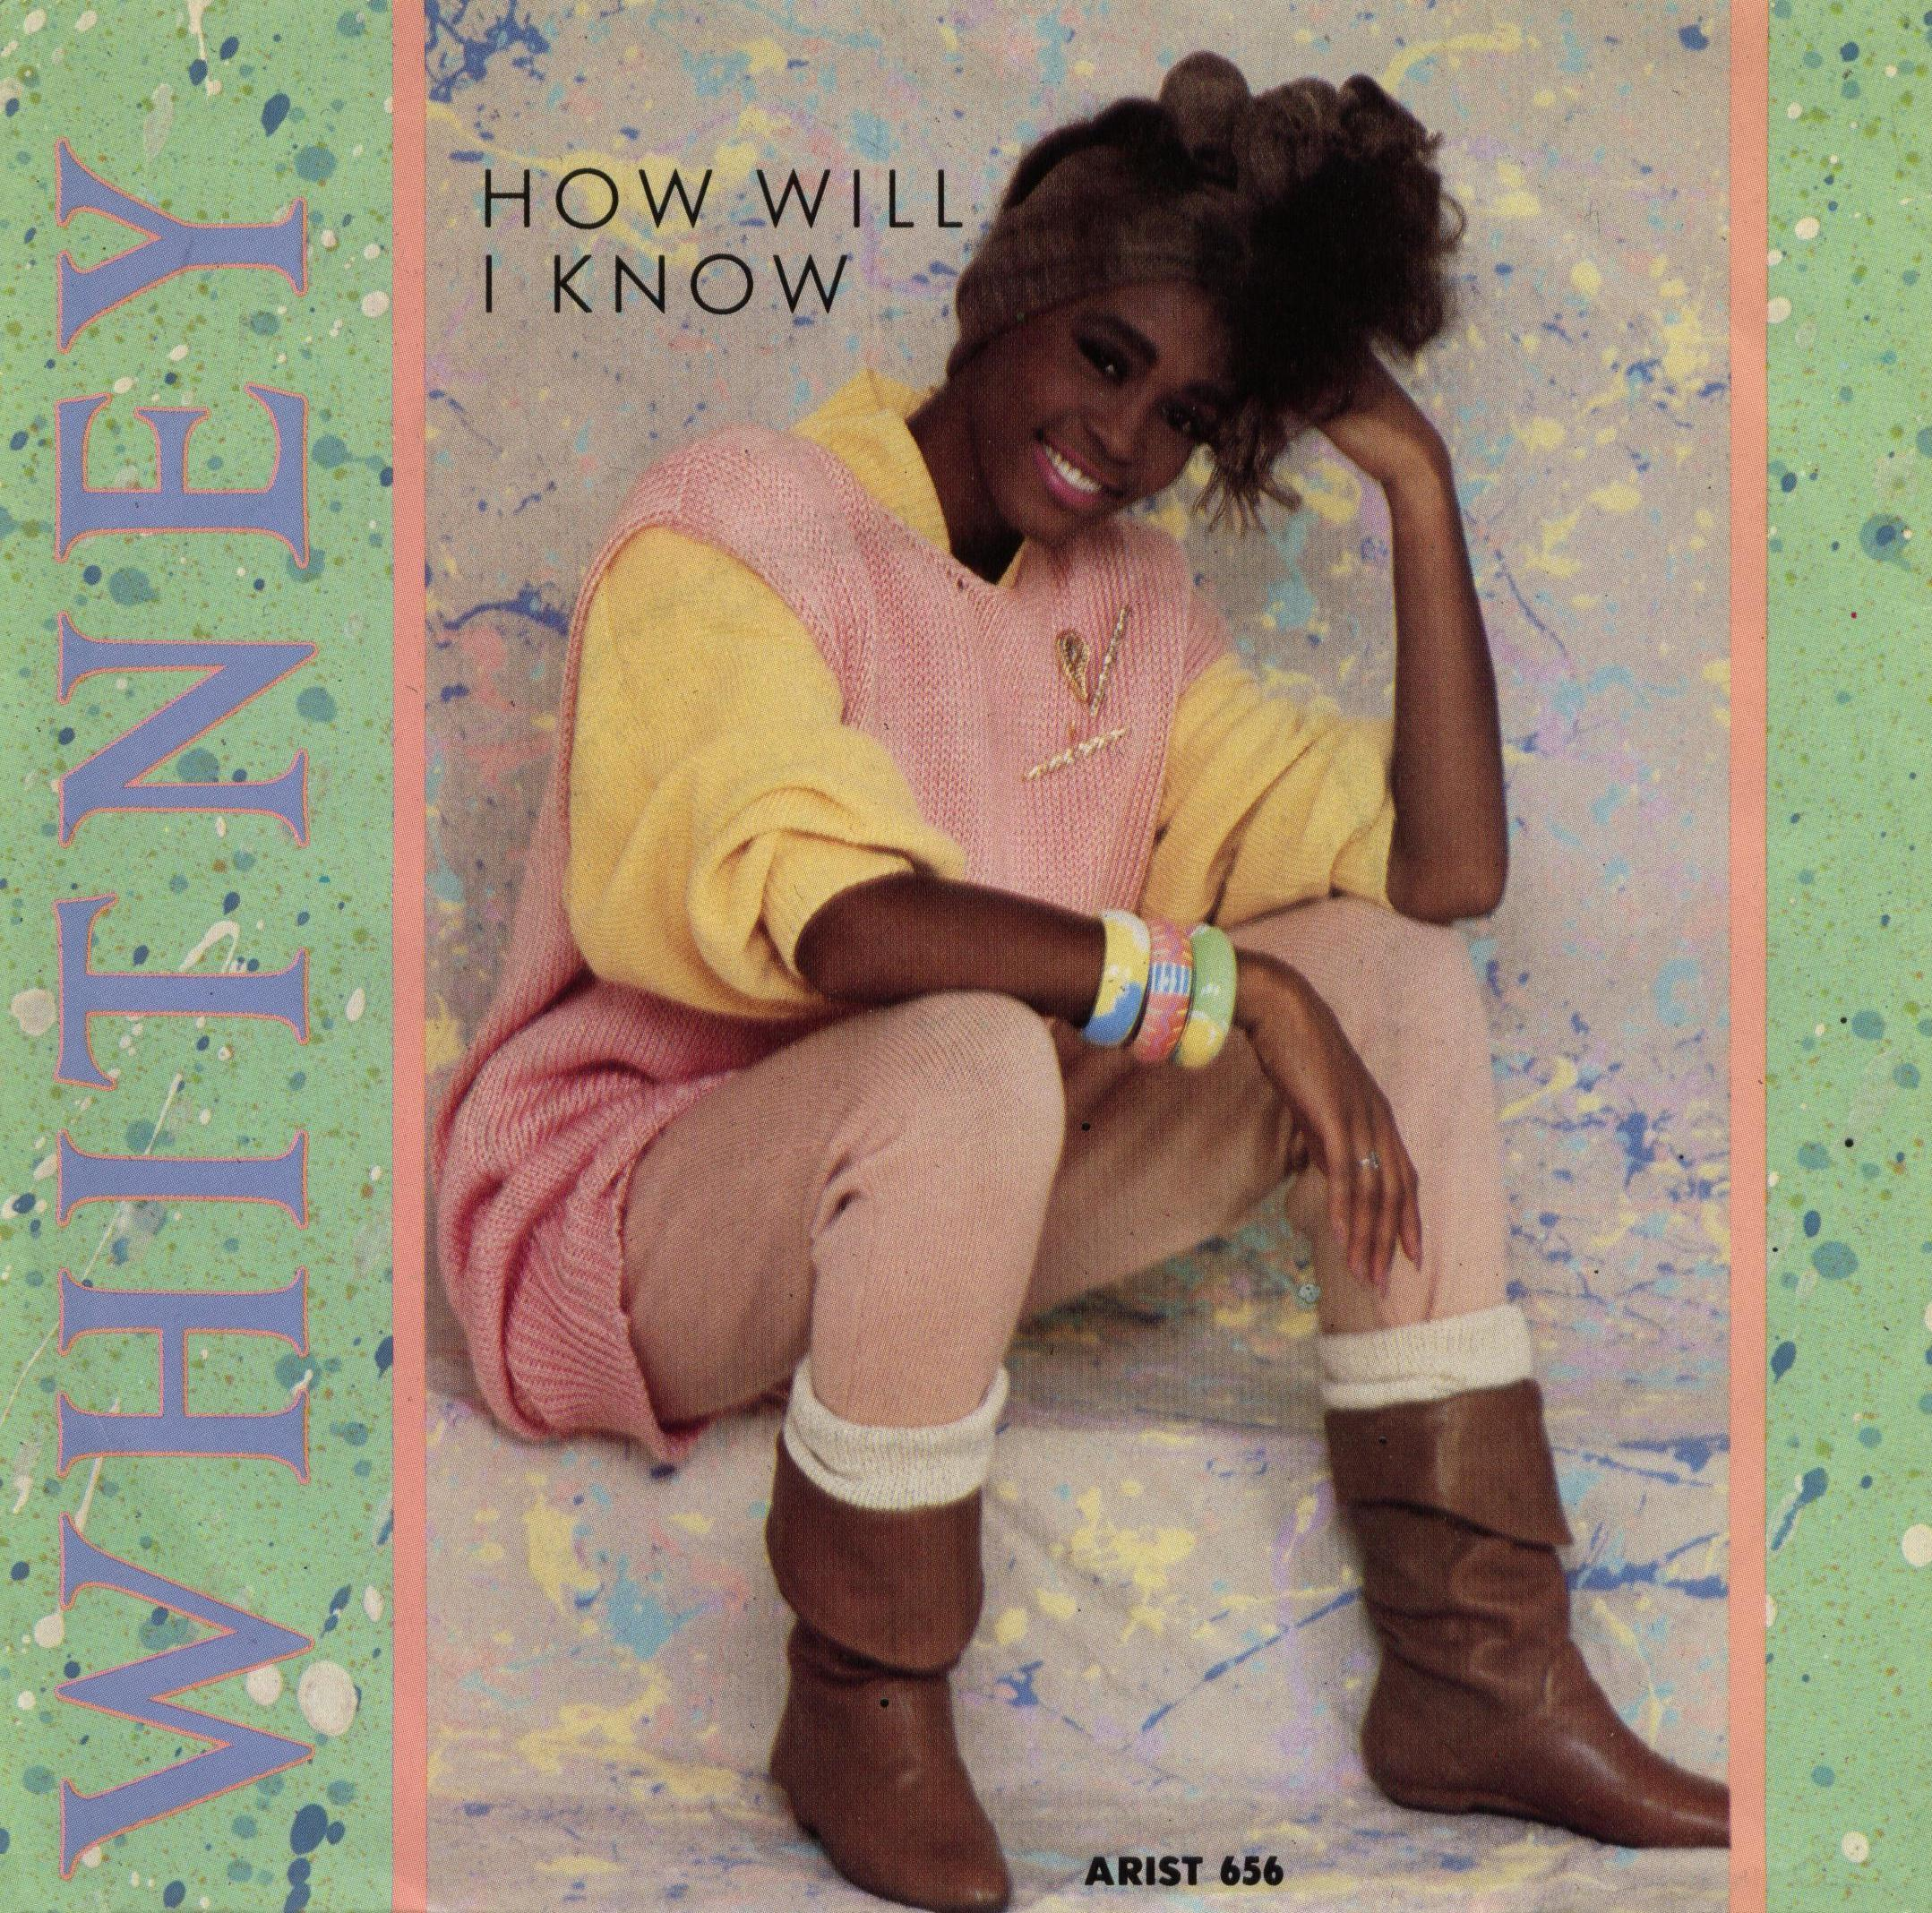
\includegraphics[scale=0.10]{img/whitney.jpg}
	\end{center}

\end{frame}
\note{
  \emph{Quickly}: Turn the \underline{benefits} just described into \underline{conditions}.
}

\section{Modeling Thought} % (fold)
\label{sec:modeling_thought}

\begin{frame}
	\frametitle{Let This Be Your Guide}
	\begin{center}
		``Modeling Thought''
	\end{center}
\end{frame}

\begin{frame}
	\frametitle{``Modeling Thought''}
	\large
	\centering{First Law of MP \\ + \\ Second Law of MP \\ = \\ }
	\vskip 0.5cm
	\begin{center}
		``Modeling Thought''
	\end{center}

	\normalsize
\end{frame}
\note{
	\begin{itemize}
		\item a conceptual rubric for evaluating when a solution calls for a metaprogrammatic solution
		\item Let's transform those motivations just mentioned into some ``Laws'' and ``Corollaries.''
	\end{itemize}
}

\subsection{Laws} % (fold)
\label{sub:laws}

\begin{frame}
	\frametitle{First Law of Metaprogramming}
	\centering{\emph{	A metaprogrammatic solution is suitable when you need to provide
	unambiguous answers (return values) to ambiguous questions (flexible /
	incomplete method calls)}
	\pause
	\vskip 0.5cm
	\centering{\emph{e.g. Rails' ORM Calculation}}
	\pause
	\vskip 0.5cm
	\begin{center}
		\emph{AKA: ``Pursuit of Insight''}
	\end{center}
}\end{frame}
\note{
	\begin{itemize}
		\item Not really ``laws''
		\item Guidelines too weak
		\item Too egotistical to call them ``Steven\'s laws of metaprogramming.''
		\item Rails
		\begin{itemize}
			\item ``Get my attributes.''
			\item Ambiguous call
			\item Always a discrete, clear, singular answer that is ``correct.''
			\item Modeling for ambiguity is hard, but Ruby makes this easy-ish
		\end{itemize}
	\end{itemize}
}


\begin{frame}
	\frametitle{Second Law of Metaprogramming}
	\centering{\emph
	{
	A metaprogrammatic solution is suitable when the mechanical recording of the
the values is time-inefficient when compared to learning the generating
heuristic.
	}
}
	\pause
	\vskip 0.5cm
	\centering{\emph{e.g. attr\_* methods}}
	\pause
	\vskip 0.5cm
	\begin{center}
		\emph{AKA: ``Avoidance of Typing''}
	\end{center}
\end{frame}
\note{
\begin{itemize}
	\item Typing a lot is a code smell
	\item Some try to fix this in IDE
	\item Others try to fix in preprocessor macros
	\item That is dumb and opaque
	\item Rubyists should eschew this
	\item An interesting tendency has emerged during my work with Ruby's MP model, and that's this first Corollary:
\end{itemize}
}

\begin{frame}
	\frametitle{First Corollary:}
	\begin{center}
		\emph{Any significant metaprogramming work undertaken to meet either of
    the laws will eventually look like it was undertaken for a reason in
    service to the opposite law}
		\pause
		\vskip 0.5cm
		\emph{Avoidance of typing reveals insight; pursuit of insight reduces typing}
	\end{center}
\end{frame}

\begin{frame}
	\frametitle{Fascinating Symmetries:  Metaprogramming and Thinking}
	Law I:  \textbf{Thinking} provides unambiguous answers to ambiguously asked things \\
	Law II: \textbf{Thinking} is the more efficient learning of generating heuristics opposed to rote recording of data \\
	\vskip 0.5cm
	This symmetry is the basis of ``Modeling Thought.''
\end{frame}

\begin{frame}
	\frametitle{``Modeling Thought:'' Born That Way}
	\begin{center}
		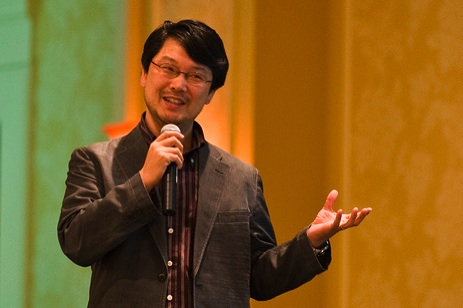
\includegraphics[scale=0.6]{img/matz.jpg}
	\end{center}
\end{frame}
\note{
And no language supports the ``modeling thought'' paradigm like Ruby.
}

\begin{frame}
	\frametitle{Stepwise Support in Ruby for ``Modeling Thought''}
	\begin{itemize}
		\item Matz' Design
		\pause
		\item Paolo's ``Spells''
		\pause
		\item A rule of thumb:  ``Modeling Thought''
		\pause
		\item Your \textbf{bold} usage
	\end{itemize}
\end{frame}
\note{
\begin{itemize}
	\item Matz made Ruby with this ``thinking'' symmetry in mind
	\item He made Ruby to be a programmer's friend
	\item Paolo distilled and named these techniques
	\item I
	\begin{itemize}
		\item I hope to provide you a rule of thumb for development
		\item I hope to give you a demo of how I used MP to tackle a non-trivial problem
	\end{itemize}
	\item I want you to use MP \textbf{boldly}
	\item Let me demonstrate my library: LatinVerb
\end{itemize}
}

\subsection{LatinVerb} % (fold)
\label{sub:_modeling_thought_in_latinverb}

\begin{frame}
	\frametitle{Demo}
	\begin{center}
		\texttt{LatinVerb}
	\end{center}
\end{frame}

\begin{frame}
	\frametitle{Just Enough Latin}
	\vskip 0.5cm
	\begin{center}
		
\includegraphics[scale=0.45]{img/captain.jpg}
	\end{center}

	\vskip 0.5cm
	\begin{center}
		\emph{``Captain!  My Captain!''}
		\vskip 0.5cm
		\copyright 1989, \emph{Dead Poet's Society}, Touchstone Pictures
	\end{center}
\end{frame}

\begin{frame}
	\frametitle{This Shouldn't Hurt{\ldots}Much}
	\begin{center}
		
\includegraphics[scale=0.45]{img/MartinWizard.jpg}
		\vskip 0.5cm
		\emph{Martin, the Wizard of Latin} \\
		\vskip 0.5cm
		\copyright 1989, \emph{The Simpsons},  20\textsuperscript{th} Century Fox
	\end{center}
\end{frame}

\begin{frame}
	\frametitle{Conjugation\ldots}
	Given the \underline{four principle parts}:  ``am\={o}, am\={a}re, am\={a}v\={\i}, amatum''
	\vskip 0.5cm
	The Specific Vector: ``Active Voice / indicative mood / present tense/ first person / singular number'' uniquely identifies:
	\vskip 0.5cm
	\begin{center}
		\emph{am\={o}}
		\vskip 0.5cm
		This process is called \underline{conjugation}.
	\end{center}
\end{frame}

\begin{frame}
	\frametitle{A Conjugation is a Unique Specification:  Stargate}
	\begin{center}
		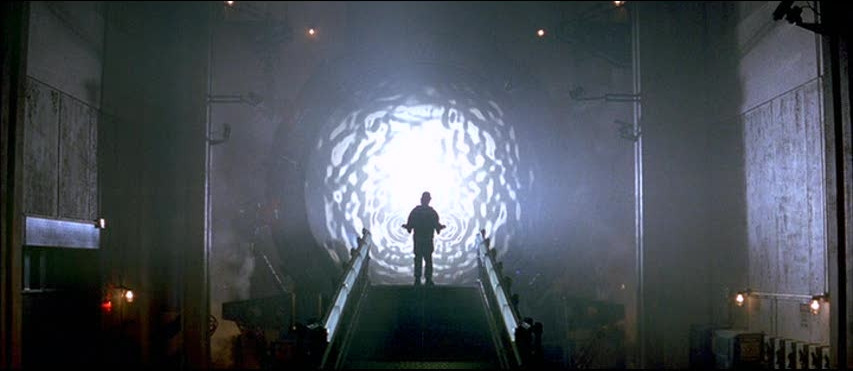
\includegraphics[scale=0.25]{img/stargate.jpg}
		\vskip 0.5cm
		6 Points in Space
		\vskip 0.5cm
		\emph{\copyright 1997, \emph{Stargate:  SG1},  MGM Worldwide Television Productions Inc.}
	\end{center}
\end{frame}

\begin{frame}
	\frametitle{Unique Specification:  Latin}
	5 Aspects
	\begin{enumerate}
		\item voice
		\pause
		\item mood
		\pause
		\item tense
		\pause
		\item person
		\pause
		\item number
		\pause
	\end{enumerate}
	\vskip 0.5cm
	A unique coordinate is a \emph{vector} or a \emph{conjugation}
\end{frame}

\begin{frame}
	\frametitle{Aggregation}
	Occasionally we want to cluster unique vectors \emph{or} leave out an aspect to get a less-granular result:
	\pause
	\begin{itemize}
		\item ``active voice indicative mood present tense'' (3 aspect, 6 reslts)
		\pause
		\item ``active voice indicative mood present tense first person'' (4 apsects, 3 results)
		\pause
		\item ``active voice indicative mood present tense first person singular number (Fully-Qualified)'' (5 aspects, 1 result)
	\end{itemize}
\end{frame}

\begin{frame}
	\frametitle{Vector Generation}
	\begin{itemize}
		\item Vector generation is a well-known, well-established, heuristically-modeled domain.
		\pause
		\item $\approx$ 2,500 years of documentation
	\end{itemize}
	\begin{center}
		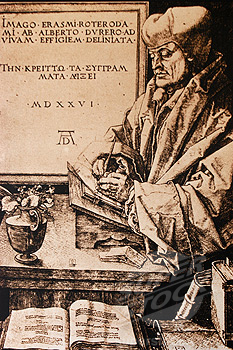
\includegraphics[scale=0.5]{img/erasmus.jpg} \\
		\pause
		\emph{``Erasmus'' by D\"{u}rer}
	\end{center}

\end{frame}

\begin{frame}
	\frametitle{Model it in Ruby!}
	\begin{center}
		
\includegraphics[scale=0.45]{img/brosh_all.png}
		\vskip 0.5cm
		\emph{Credit:  Allie Brosh}
	\end{center}
\end{frame}

\begin{frame}
	\frametitle{Or as Aaron Patterson once said:}
	\begin{center}
		``Do something worthless of questionable value.'' \\ -- \emph{Aaron Patterson}
	\end{center}
\end{frame}
\note{
So, let's talk about how I went about modeling this problem.  Here's a specification.
}


\begin{frame}
	\frametitle{LatinVerb's Purpose}
	LatinVerb should be a library for conjugating Latin verbs provided their ``four principle parts (am\={o}, am\={a}re, am\={a}v\={\i}, amatum).''
	\pause
	\vskip 0.5cm
	Vectors should be accessed by pretty method calls like:
	\vskip 0.5cm

	\texttt{active\_voice\_indicative\_mood\_present\_tense{\ldots}\\
	\_first\_person\_singular\_number}

\end{frame}

\begin{frame}
	\frametitle{Painful Combinations}
	\begin{itemize}
		\item 6 results means 6 methods to be defined \emph{per tense}
		\pause
		\item \ldots $\times$ 6 tenses (present/imperfect/future/perfect/past-perfect/future-perfect)
		\pause
		\item \ldots $\times$ 2 voices (active/present)
		\pause
		\item \ldots \emph{and then there's another mood with 4 tenses of its own!}
		\pause
		\item Each regular Latin verb has $\approx$  160 unique vectors
		\pause
		\item There are 5 standard paradigms
		\pause
		\item \ldots and at least $1,000$ verbs
	\end{itemize}
\end{frame}

\begin{frame}
		\frametitle{Pain}
		\begin{itemize}
			\item Typing all of these several hundred(thousand?)-odd values for \emph{fully-specified} vectors would definitely hurt
			\pause
			\item What if you had \emph{incomplete} data per our Aggregation section?  4/5 of the vector specification?  3/5?  Write \emph{yet} even more methods
		\end{itemize}
		\begin{center}
			\begin{tabular}{|c|c|c|}
				\hline
				  & Singular Number &  Plural Number\\
				\hline
				First Person  & laud\={o}  & laud\={a}mus\\
				Second Person & laud\={a}s & laudatis \\
				Thrid Person  & laudat     & laudant \\
				\hline
			\end{tabular}
		\end{center}
\end{frame}

\begin{frame}
	\frametitle{Metaprogramming Makes a Saving Throw!}
	\begin{center}
		Law II says to MP our way out of the pain
		\vskip 1.0cm
		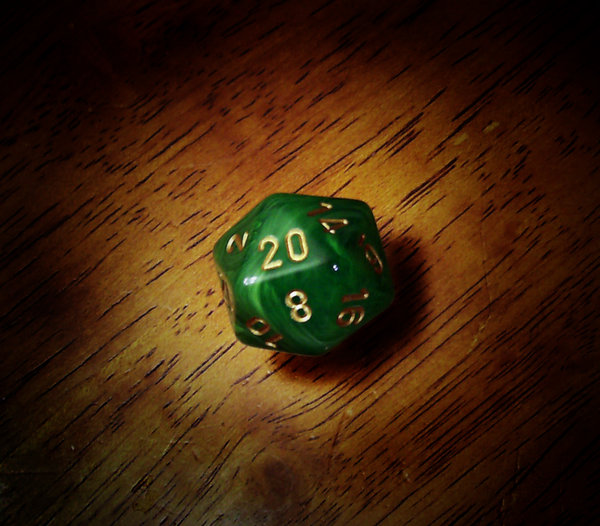
\includegraphics[scale=0.25]{img/natural_20.jpg} \\
		\emph{Credit: Marco26 on DeviantArt}
	\end{center}
\end{frame}

\begin{frame}
	\frametitle{Specification}
	Take an array of elements and tack them onto a base, derived from the given, second part, with the results returned as an array.  Sub-specify by \underline{person} (1, 2, 3) and/or \underline{number} or cluster by either.
	\pause
	\vskip 0.5cm
	\emph{Why does that sound familiar?}
	\vskip 0.5cm
	
\includegraphics[scale=0.45]{img/determined.png}
\end{frame}


\begin{frame}
	\frametitle{Translating a Domain Problem to Ruby (1/3)}
	\emph{Take an array of elements and tack them onto a base, derived from the
    given, with the results returned as an array.
}	\begin{center}
		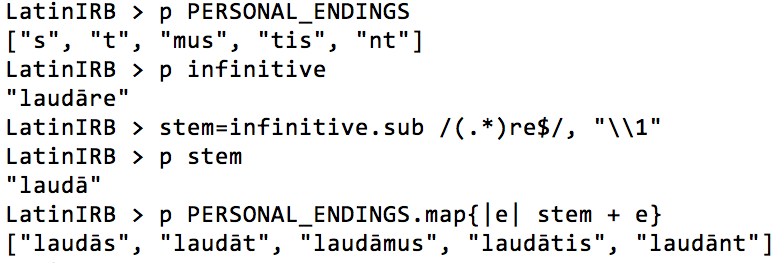
\includegraphics[scale=0.38]{img/conj_how.png}
	\end{center}
\end{frame}

\begin{frame}
	\frametitle{Translating a Domain Problem to Ruby (2/3)}
	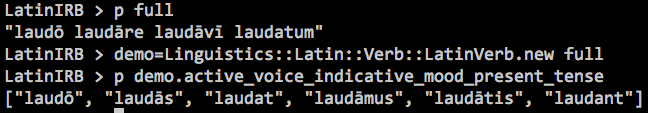
\includegraphics[scale=0.39]{img/conj_how_3b.png}
\end{frame}


\begin{frame}
	\frametitle{Translating a Domain Problem to Ruby (3/3)}
	\emph{
		Sub-specify by \underline{person} (1, 2, 3) or \underline{number} or
    cluster by either. \\
		\pause
		{\ldots} and allow terms in method call to be reordered
  }
	\vskip 0.5cm
	\begin{center}
		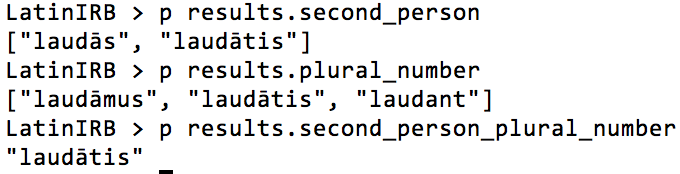
\includegraphics[scale=0.38]{img/conj_subspec.png}
	\end{center}
\end{frame}

\begin{frame}
	\frametitle{MP Provides:  Massive Laziness Win}
	\begin{itemize}
		\item $\approx$ 48 methods covered; 6 written
		\pause
		\item 2 aspects in play
		\pause
		\item One reponse class (\texttt{TenseBlock})
	\end{itemize}
\end{frame}

\begin{frame}
	\frametitle{Scale it Up!: Dynamic Dispatch in \texttt{method\_missing}}
	\begin{center}
		\emph{Be flexible on all 5 aspects}
	\end{center}
	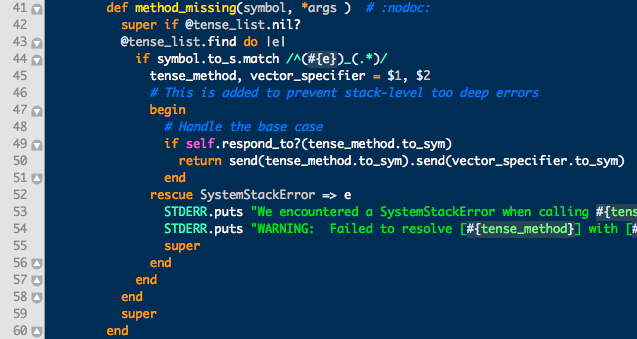
\includegraphics[scale=0.45]{img/lv_mm.png}
\end{frame}
\note{
The same technique that we used with a Tense Block that gave each one several extra methods, I then scaled that shortcut by doubling the dynamic method call.
}

\begin{frame}
	\frametitle{Result:  Super-Massive Laziness Win}
	\begin{itemize}
		\item Covered the thousands of methods predicted
		\pause
		\item \ldots and provided the clustering methods as well as a surprising bonus
	\end{itemize}
	\pause
	\vskip 0.5cm
	\emph{I only wrote 24 methods}
\end{frame}

\begin{frame}
	\frametitle{Benefits via Law II}
	\begin{itemize}
		\item Saved many keystrokes by writing using a \underline{Ghost Method}
		\pause
		\item Saved creating \textbf{\$A\_LOT\_OF} additional methods -- \emph{many of which I didn't even think of!}
	\end{itemize}
\end{frame}

\begin{frame}
	\frametitle{The Corollary Emerges}
	\begin{itemize}
		\item 	Pursued ``less typing'' but wound up with ``respond to ambiguous calls with unambiguous data''
		\pause
		\item  \emph{Insights Emerged!}:  `Modeling Thought'' yields many of these surprises
	\end{itemize}
\end{frame}


\begin{frame}
	\frametitle{Law I Emerges{\ldots}With Surprises}
	\begin{itemize}
		\item 5 additional ``aggregate methods'' per tense emerged
		\begin{itemize}
			\item {aTenseBlock}.singular\_number (\texttt{3 results})
			\item {aTenseBlock}.first\_person (\texttt{2 results})
		\end{itemize}

		\pause

		\item Flexible word order \emph{emerged} that did the right thing
		\begin{itemize}
			\item first\_person\_singular\_number
			\item singular\_number\_first\_person
		\end{itemize}

		\pause

		\item Avoided Java-ish paramteterized brain damage
	\end{itemize}
\end{frame}


\begin{frame}
	\frametitle{Java-ish Brain Damage:  Parameterization}
 	\texttt{String calculate\_vector(VerbyType aV, String v, String m, String t, String p, String n)}
	\vskip 0.5cm

	\begin{center}
		\textbf{OR}
	\end{center}

	\vskip 0.5cm
	\texttt{Object[] calculated\_values = \{aV, v, m, t, p, n\};}
	\texttt{String calculate\_vector(calculated\_values)};
\end{frame}
\note
{A particular reason that I want to highlight this benefit is because Java/C-style
parameterization is not how we think.
}

\begin{frame}
	\frametitle{anti-Parameterization:  Not How We Think, Not Modeled Thought}

		\begin{center}
			
\includegraphics[scale=0.15]{img/SubwayLogo.png}
		\end{center}

	\begin{itemize}
		\item We \emph{do not} think like we are ordering from Subway.
		\pause
		\item NO:  \emph{``I'll have a sandwich:  bread is rustic Italian, meat is salami, cheese is provelone, veggies are an array of lettuce, tomato \ldots''}
		\pause
		\item YES:  \emph{``I'll have an Italian on rustic Italian with salami and provelone and from the veggie bin, lessee, lettuce and tomato\ldots''}
	\end{itemize}

\end{frame}
\note{This is probably something \emph{right} about the Objective-C language.}

\begin{frame}
	\frametitle{Pretty Parameterization}
	\texttt{instance.active\_voice\_indicative\_mood\_present\_tense}
	\begin{center}
		\textbf{NOT}
	\end{center}
	\texttt{instance.calculate\_vector('active','indicative')} \ldots
\end{frame}

\begin{frame}
	\frametitle{Clarity \& Communication}
	\begin{center}
		\emph{``Code that Communicates''}
		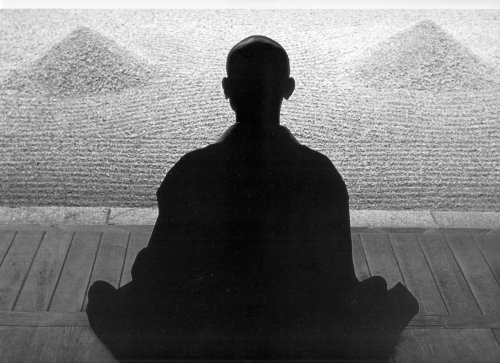
\includegraphics[scale=0.45]{img/Zen04.jpg}
	\end{center}
\end{frame}

\begin{frame}
	\frametitle{Pause for ``applause''}
	\begin{center}
		\texttt{LatinVerb:  Demo End}
		\pause
		\vskip 0.5cm
		\emph{FYI:  Applause is derived from our example word ``laud\={a}re'' meaning ``to praise'' literally meaning ``to praise toward''}
	\end{center}
\end{frame}

\begin{frame}
	\frametitle{What MP Techniques Make This Possible?}
	\begin{center}
		HOW?
	\end{center}
\end{frame}
\note{
If I were to send you home with anything, I want you to go home with the ``Modeling Thought'' guideline and the knowledge
of all the spell defined by Perrotta.  But I know you want a few code samples, so let me provide them.

Provided:
\begin{enumerate}
	\item Open Class
	\item Kernel Method
	\item Singleton Method
\end{enumerate}

Here are the next tier of spells, and they happen to be what enabled LatinVerb's flexibility.
}


\subsection{MP Techniques} % (fold)
\label{sub:methods}

\begin{frame}
	\frametitle{\underline{Ghost Method} in \texttt{TenseBlock}}
	\begin{center}
		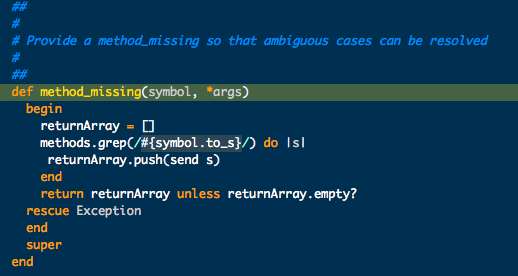
\includegraphics[scale=0.45]{img/tenseblock_mm.png}
	\end{center}

\end{frame}

\begin{frame}
	\frametitle{MP Techniques Used:  Second-Degree Spells}
	\begin{enumerate}
		\item \underline{Blank Slate}:  A TenseBlock is a Blank Slate, effectively
		\item \underline{Ghost Method}:  Dont define a method (in \texttt{TenseBlock}) so that its \texttt{method\_missing} acts as \texttt{method\_called} for dispatching
		\item \underline{Dynamic Dispatch}:  \texttt{self.send} in \texttt{TenseBlock}
	\end{enumerate}
\end{frame}

\begin{frame}
	\frametitle{Third-Degree Spells}
	\begin{itemize}
		\item Dynamic Method
		\item Around Alias
		\item DSL:  \emph{See Evan's talk!}
		\item Class Extension a.k.a. Mixin
	\end{itemize}
\end{frame}

\begin{frame}
	\frametitle{Conclusion:  Goals Into Action!}
	\begin{enumerate}
		\item \textbf{Let's provide a clearer path to learning} MP in the Ruby community \ldots
		\pause
		\item \textbf{since we know we} can't \emph{not} learn this.
		\pause
		\item \textbf{Since we know when we} should reach for the MP ``hammer'' \textbf{thanks to the ``modeling thought'' guideline}
		\pause
		\item \textbf{and have a demonstrated} example of thinking in terms of MP
		\pause
		\item \textbf{we will} use MP \textbf{boldly}
	\end{enumerate}
\end{frame}
% section modeling_thought (end)

\section{Supplementary} % (fold)
\label{sec:supplementary}

\begin{frame}
	\frametitle{Supplementary}
	\begin{center}
		Supplementary Information
	\end{center}
\end{frame}

\begin{frame}
	\frametitle{Book}
	\underline{Metaprogramming Ruby} by Paolo Perrotta
\end{frame}

\begin{frame}
	\frametitle{List of Spells}
	\texttt{http://ducktypo.blogspot.com/2010/\\08/metaprogramming-spell-book.html}
\end{frame}

\begin{frame}
	\frametitle{(Meta)programming Politely}
	\texttt{http://confreaks.net/videos/\\374-rubyconf2010-the-polite-programmer-s-guide-to\\-ruby-etiquette}
\end{frame}

\begin{frame}
	\frametitle{Photo Credits}
	\begin{enumerate}
		\footnotesize
		\item ``Zen'' pic:\\ \texttt{http://www.insidesocal.com/tomhoffarth/archives/2011\\
		 /06/shawn-greens-ze.html}
		\normalsize
	\end{enumerate}
\end{frame}

\begin{frame}
	\frametitle{Colophon}
	\LaTeX and the Beamer Slide Toolkit
\end{frame}

\begin{frame}
	\frametitle{SpeakerRate}
	\centering{Help Me Get Better!}
	\vskip 1.25cm
	\centering{\texttt{http://speakerrate.com/talks/\\7831-practical-metaprogramming-modeling-thought}}
\end{frame}

\begin{frame}
	\frametitle{Contact Me! (Again)}
	\begin{center}
		Steven G. Harms \\
		\vskip 1.25cm
		Physically:  San Francisco, CA\\
		Email:  \texttt{lsrcv@sgharms.oib.com} \\
		Twitter / GitHub:  \texttt{sgharms} \\
		G+
	\end{center}
\end{frame}

\end{document}

